\chapter{Methods}

\begin{figure}
    \centering
    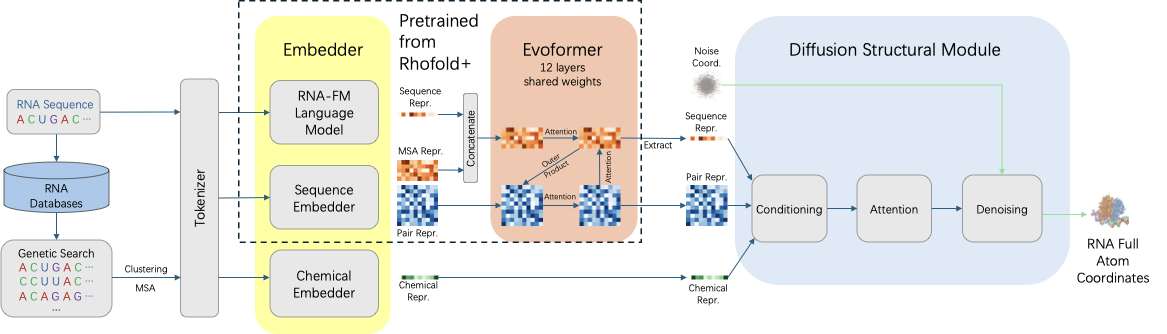
\includegraphics[width=1\linewidth]{img/Architecture.png}
    \caption{Overview of the Diffold framework}
    \label{fig:architecture}
\end{figure}

\section{MSA Feature Generation}
In this study, the model uses multiple sequence alignment (MSA) features to capture evolutionary information among RNA sequences. For each target RNA sequence, we perform a remote BLASTN search against the NCBI nucleotide (nt) database using the BLAST “QBlast” Common URL API provided by NCBI. The QBlast API is an HTTP-based programmatic interface to the NCBI BLAST servers, allowing automated submission of search queries, retrieval of job status, and downloading of alignment results without manual intervention. In our implementation, we adopt the “Put/Get” workflow of the Common URL API to submit each query sequence, parse the returned results, and rank the obtained homologous sequences based on E-value and bit score\cite{altschul1990blast, altschul1997gappedblast}. Due to hardware memory limitations, we retain up to 250 non-redundant homologous sequences as the maximum MSA depth. In contrast to models such as AlphaFold2 and RhoFold+, which rely on different MSA construction tools and databases, our approach uses QBlast for remote retrieval\cite{Jumper2021AlphaFold}. Following sequence retrieval, we apply the same alignment and feature-construction procedures as RhoFold+ to build the MSA, from which we extract per-position MSA profiles and pairwise co-evolutionary features as input to the Rhoformer backbone. Compared to maintaining a local BLAST database, using QBlast simplifies deployment and ensures continuous access to the most up-to-date NCBI nt database.

\section{Embedder}

Our model adopts a token-based feature embedding strategy, where each token corresponds to a nucleotide residue in the RNA sequence. The embedding module consists of two core components: token embedder and atom embedder.
\subsection{Token Embedder}
\subsubsection{MSA Embedder}

This module receives a multiple sequence alignment (MSA) as input, with shape $\mathbb{R}^{B \times K \times L}$, where $B$ denotes the batch size, $K$ the number of aligned sequences, and $L$ the sequence length. A learnable token embedding layer maps discrete nucleotide tokens into a 256-dimensional continuous vector space. To capture positional information, we apply a learned positional embedding that supports maximum sequence lengths up to 4096.

To construct pairwise representations, we adopt an outer-product–style strategy: given a sequence embedding $e \in \mathbb{R}^{L \times d}$, the pairwise representation is formed by concatenating embeddings at positions $i$ and $j$, namely
$p_{ij} = [\, e_i \oplus e_j \,],$
where $\oplus$ denotes the concatenation operation. A linear projection followed by 2D sinusoidal positional encoding yields the final pairwise feature tensor $\mathbf{Z} \in \mathbb{R}^{L \times L \times 128}$.

Meanwhile, we use the pretrained RNA language model RNA-FM to enhance representational capacity\cite{Chen2022RNAFM}. RNA-FM is based on a 12-layer Transformer architecture and is pretrained on large-scale RNA sequence corpora, providing a 640-dimensional single-sequence representation $\mathbf{S}_{\text{RNA-FM}}$. Through feature concatenation and linear dimensionality reduction, we fuse RNA-FM features with MSA-derived embeddings:
$$\mathbf{M} = \text{Linear}\left([\mathbf{M}_{\text{MSA}} \oplus \mathbf{S}_{\text{RNA-FM}}]\right)$$

\subsubsection{Recycling Embedder}
Inspired by the recycling mechanism of AlphaFold2, this module incorporates predictions from the previous iteration as additional input for the current iteration. Given the single representation $\mathbf{s}^{(t-1)} \in \mathbb{R}^{L \times 256}$, pair representation $\mathbf{z}^{(t-1)} \in \mathbb{R}^{L \times L \times 128}$, and the predicted C1′ atomic coordinates $\mathbf{x}^{(t-1)}_{\text{C1}'} \in \mathbb{R}^{L \times 3}$ from iteration $t-1$, the recycling embedder first converts coordinates into a distance-histogram representation:
$$d_{ij} = \text{OneHot}\bigl(\|\mathbf{x}_i - \mathbf{x}_j\|_2,\ \text{bins} = [2, 22]\ \text{\AA}\bigr)$$
The 15-dimensional binned distances are then projected to 128 dimensions via a linear layer and added to the normalized pairwise features. The MSA features are layer-normalized and added to the first row of the current MSA representation.
This design allows the model to inject geometric constraints across recycling iterations, enabling progressive refinement of predicted structures.

\subsection{Atom Embedder}


Unlike traditional token-level representations, our model adopts an atom-level embedding strategy to capture finer-grained intramolecular interactions. This module follows Algorithm 2 of AlphaFold3, transforming raw atomic coordinates into multi-scale hierarchical representations.

  
\subsubsection{Atomic Feature Initialization}

Given the atomic coordinates $\mathbf{a} \in \mathbb{R}^{N_{atom} \times 3}$ and atom-pair relations $\mathbf{p} \in \mathbb{R}^{N_{atom} \times N_{atom} \times 5}$ (where  is the total number of atoms), we apply bias-free linear layers to map inputs into the embedding space: $$\mathbf{A}^{(0)} = W_a \mathbf{a},\quad \mathbf{P}^{(0)} = W_p \mathbf{p},$$
where atomic features are 128-dimensional and pairwise features are 16-dimensional.

  
\subsubsection{Atom Representation Conditioning}
To enhance expressiveness of pairwise features, we introduce a node–edge conditioning mechanism. For each atomic feature, an MLP produces a modulation signal:

$$\mathbf{c} = \text{ReLU}\left(\text{Linear}\left(\text{LayerNorm}(\mathbf{A}^{(0)})\right)\right) \in \mathbb{R}^{N_{atom} \times 32}$$

The vector $\mathbf{c}$ is split into row- and column-wise modulation terms $\mathbf{c}_{\text{row}}$ and $\mathbf{c}_{\text{col}}$ (each 16-dimensional), which are added to the windowed pairwise features, enabling atomic properties to modulate atom–atom interactions.

  
\subsubsection{Windowed Atomic Transformer}

To support large molecular systems that may contain thousands of atoms, we apply a sliding-window mechanism that partitions the atom sequence into $N_w$ windows of size $w = 27$. Within each window, a Diffusion Transformer layer performs self-attention:

$$\mathbf{A}^{(l+1)} = \text{DiffusionTransformer}^{(l)}\bigl( \mathbf{A}^{(l)},\ \text{single} = \mathbf{A}^{(l)},\ \text{pairwise} = \mathbf{P}^{(l)} \bigr),$$

for $l \in {1, 2, 3}$. Each layer contains four attention heads and learns local atomic interaction patterns.

The windowing strategy reduces computational complexity from $O(N_{atom}^2)$ to $O(N_{atom} \cdot w)$, making it feasible to model large ligand–RNA complexes.

  
\subsubsection{Atom-to-Token Pooling}

Since functional units of biomolecules typically act at the residue (token) level rather than the atom level, we aggregate atom-level embeddings into token-level features via masked average pooling.
Let $N_{\text{atom}}$ denote the number of atoms and $L$ the number of tokens (residues).
We define an atom mask $\mathbf{m}_a \in \{0,1\}^{N_{\text{atom}}}$ and an atom-to-token assignment vector
$\mathbf{g} \in \{1,\dots,L\}^{N_{\text{atom}}}$, where $g_j$ indicates the token index to which atom $j$ belongs.
Accordingly, the set of atoms assigned to token $i$ is
\[
\mathcal{A}(i) = \{\, j \in \{1,\dots,N_{\text{atom}}\} \mid g_j = i \,\}.
\]
Given atom embeddings $\mathbf{h}^{\text{atom}}_j \in \mathbb{R}^{d_a}$, the pooled token feature $\mathbf{T}_i \in \mathbb{R}^{d_a}$ is computed as
\[
\mathbf{T}_i
= \frac{\sum_{j \in \mathcal{A}(i)} m_a[j]\;\mathbf{h}^{\text{atom}}_j}
       {\sum_{j \in \mathcal{A}(i)} m_a[j] + \varepsilon},
\]
where $\varepsilon>0$ is a small constant to avoid division by zero when a token has no valid atoms after masking.


  

The embedder outputs a named tuple consisting of:

1. $\mathbf{A}^{B \times N_{atom} \times 128}$ — atom-level features,
    
2. $\mathbf{P}^{B \times N_w \times w \times 16}$ — windowed pairwise features, $N_w$ denotes the number of windows.
    

This hierarchical design enables the model to capture molecular interactions at atomic resolution while performing efficient global reasoning at the token level, achieving a balance between computational efficiency and modeling fidelity.

\section{Rhoformer}

We adopt the Rhoformer architecture from RhoFold+ as the backbone network\cite{Shen2024RhoFoldPlus}, which is responsible for integrating evolutionary information with structural constraints. The module takes as input the MSA representation $\mathbf{M} \in \mathbb{R}^{B \times K \times L \times 256}$ and the pair representation $\mathbf{Z} \in \mathbb{R}^{B \times L \times L \times 128}$, and updates them through 12 stacked Rhoformer blocks.

  

Each block consists of two update stages.

(1) MSA update stage. Row attention with pair bias and column attention are applied to capture both intra-sequence dependencies and cross-sequence coevolutionary signals.

(2) Pair update stage. The module performs outer-product mean, triangle multiplicative updates, triangle attention, and a transition feed-forward network, which collectively project information from the MSA space into the residue-pair space and strengthen geometrical consistency. Bidirectional information flow between the MSA and pair representations is maintained through pair biases and outer-product operations.

After 12 update blocks, the single-sequence representation is extracted from the first row of the MSA (corresponding to the query sequence) as

$$\mathbf{S} = \text{Linear}(\mathbf{M}[0]) \in \mathbb{R}^{B \times L \times 256},$$

which is then fed, together with the refined pair representation, into the subsequent Structure Module. All submodules employ residual connections and layer normalization to stabilize the training of deep networks. To reduce memory consumption for long sequences, we additionally apply gradient checkpointing and a dynamic chunking mechanism.

\section{Diffusion Structural Module}

Diffusion models are a class of generative models grounded in stochastic differential processes\cite{sohldickstein2015diffusion, ho2020ddpm}. Their core idea is to gradually perturb the data distribution into an isotropic Gaussian distribution through a forward noising process, and to learn a reverse denoising process that progressively recovers samples consistent with the target distribution starting from random noise. Unlike conventional direct regression-based generative models, diffusion models represent complex high-dimensional distributions through multi-step iterative refinement, which has demonstrated superior stability and diversity in structural generation tasks.

In the task of RNA three-dimensional structure prediction, we treat the molecular 3D atomic coordinates as the data to be modeled. Let the ground-truth atomic coordinates be denoted as  $\mathbf{x}_0 \in \mathbb{R}^{N_{atom} \times 3}$,  where $N_{atom}$ represents the total number of atoms in the molecule.

The diffusion process can be conceptually divided into two stages, forward diffusion process and reverse denoising process.

The forward diffusion process gradually corrupts the original data by adding Gaussian noise, mapping clean samples into a family of noisy distributions. For any continuous noise level $\sigma > 0$, the forward process is defined as

$$  
\mathbf{x}_\sigma = \mathbf{x}_0 + \sigma \boldsymbol{\epsilon},  
\quad \boldsymbol{\epsilon} \sim \mathcal{N}(\mathbf{0}, \mathbf{I}),  
$$

where $\mathbf{x}_\sigma$ denotes the perturbed coordinates at noise scale $\sigma$. As $\sigma$ increases, the data distribution progressively approaches an isotropic Gaussian distribution; in the limit $\sigma \to \infty$, the samples contain almost no structural information. This continuous formulation of noise injection avoids the explicit Markov chain construction used in discrete-time diffusion models, providing a convenient foundation for designing stable reverse processes.


The reverse denoising process makes the generative capability of diffusion models, which aims to progressively recover the original data $\mathbf{x}_0$ from noisy samples $\mathbf{x}_\sigma$. This process can be interpreted as iterative denoising in noise-scale space, moving from higher noise levels toward lower ones.

In theory, the reverse process corresponds to a conditional distribution
$$  
p(\mathbf{x}_{\sigma'} \mid \mathbf{x}_\sigma),  
\quad \sigma' < \sigma,  
$$
whose exact form is generally intractable. In practice, this distribution is approximated using a neural network.

Specifically, diffusion models train a parameterized denoising network $\mathbf{D}_\theta$ that predicts a denoised estimate given noisy coordinates and the corresponding noise level:

$$  
\hat{\mathbf{x}}_0 = \mathbf{D}_\theta(\mathbf{x}_\sigma, \sigma).  
$$

This network effectively learns the conditional expectation of the data distribution across noise scales, enabling structure correction at arbitrary noise levels.

\begin{figure}
    \centering
    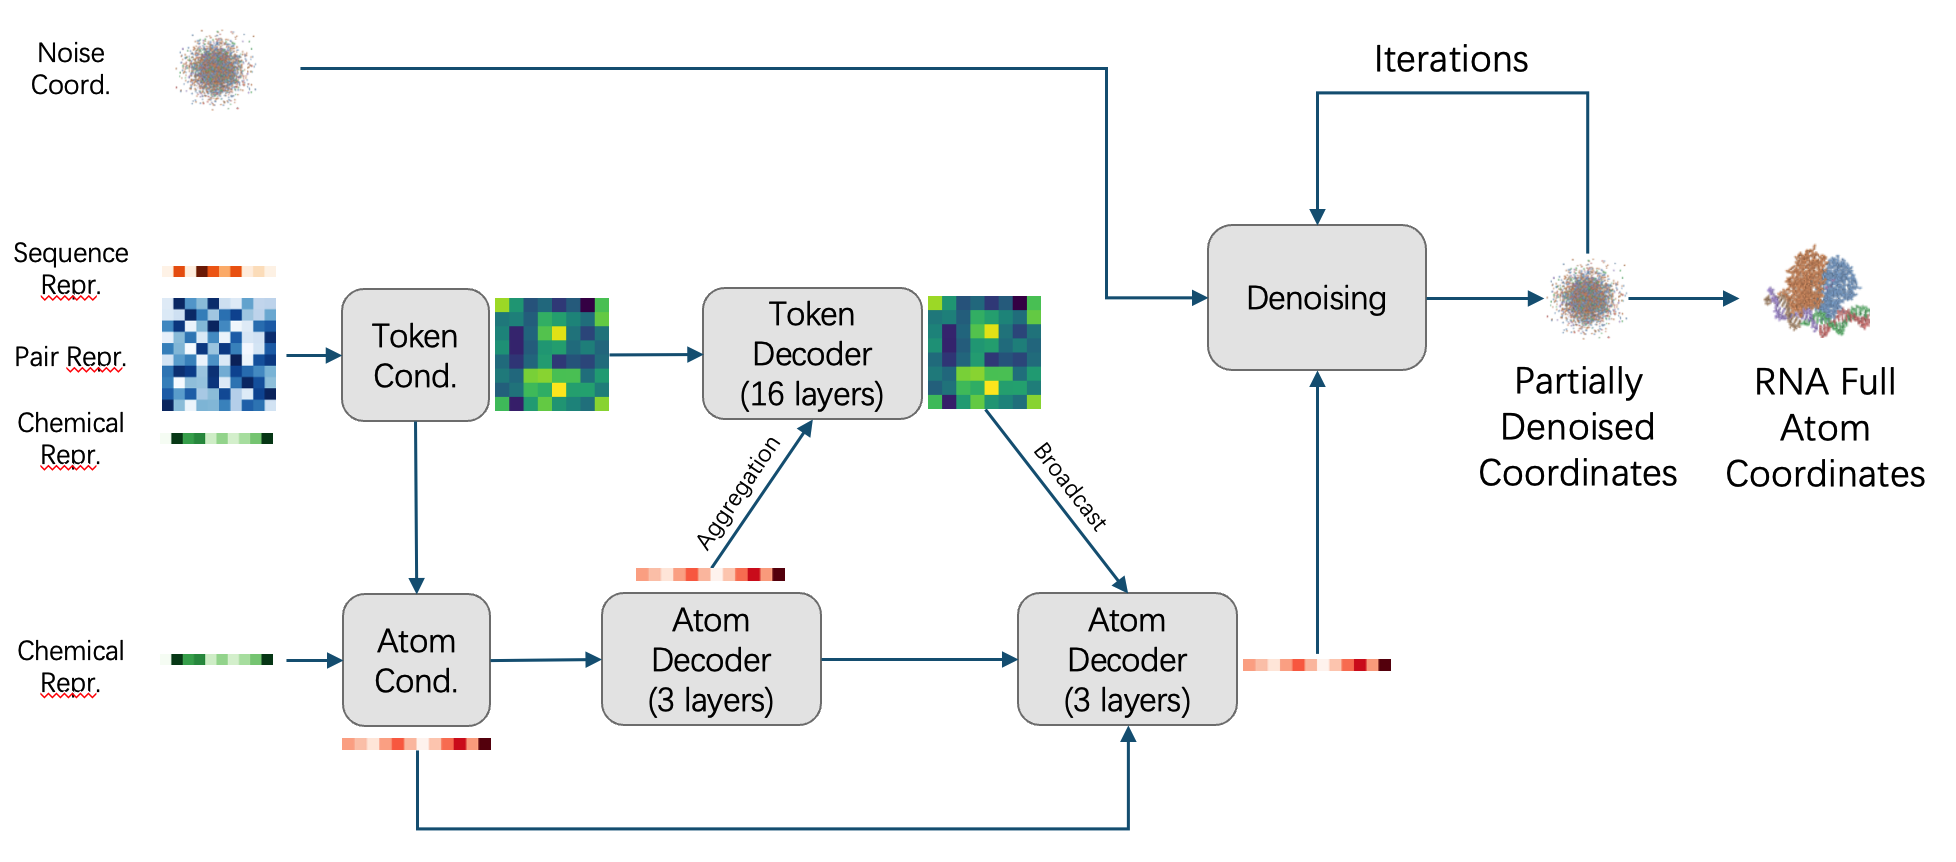
\includegraphics[width=1\linewidth]{img/Diffusion_module.png}
    \caption{Overview of the diffusion structural module. Noisy atom coordinates are iteratively refined by a token-level decoder and an atom-level decoder with bidirectional aggregation and broadcasting. Sequence/pair representations and chemical features are injected via token/atom conditioning to produce full-atom RNA coordinates.}
    \label{fig:diffusion module}
\end{figure}

\subsection{Conditional Diffusion Modeling}

In RNA structure prediction, the generated three-dimensional conformations must be consistent with given biological conditions, such as sequence information, evolutionary constraints, and chemical structure features. Therefore, the denoising network is formulated as a conditional model:

$$  
\hat{\mathbf{x}}_0 = \mathbf{D}_\theta(\mathbf{x}_\sigma, \sigma \mid \mathcal{C}),  
$$

where $\mathcal{C}$ denotes the set of all conditional inputs, including residue-level representations, atomic features, atom-pair relationships, and masking information.

During training, the model minimizes the discrepancy between predicted and ground-truth coordinates across different noise levels, learning to leverage conditional information to progressively remove noise and recover physically plausible 3D structures. During inference, the model starts from Gaussian noise and iteratively applies the reverse denoising process to generate the final structure.


\subsection{Elucidated Diffusion Model（EDM)}


In this study, we adopt the Elucidated Diffusion Model (EDM) framework proposed by Karras et al. to perform diffusion modeling of atomic coordinates\cite{Karras2022EDM}. Compared to conventional DDPM-style approaches, EDM treats the continuous noise level $\sigma$ as a core variable and unifies learning across different noise scales via a preconditioning mechanism, leading to improved training stability and sampling efficiency.

During training, noisy samples are constructed from the ground-truth coordinates $\mathbf{x}_0$ as

$$  
\mathbf{x} = \mathbf{x}_0 + \sigma \boldsymbol{\epsilon}, \qquad \boldsymbol{\epsilon} \sim \mathcal{N}(\mathbf{0}, \mathbf{I}),  
$$

and the model learns a noise-conditioned denoising mapping that exhibits consistent recovery capability across multiple noise scales.

\subsection{Token–Atom Hierarchical Denoising Architecture}

The core of the diffusion model is the denoising network $\mathcal{F}_\theta$, whose objective is to recover physically plausible molecular conformations from noisy structures under a given noise level. To address the hierarchical nature of RNA structures—characterized by both atom-level local geometric constraints and residue-level long-range interactions—we employ a Token–Atom hierarchical denoising architecture inspired by AlphaFold3. This design models structural information at multiple scales, achieving a balance between computational efficiency and modeling accuracy.

Biomolecular structures such as RNA and proteins exhibit intrinsic hierarchy. At the microscopic scale, bond lengths, bond angles, and non-bonded interactions govern local geometric stability; at higher levels, residue stacking, secondary structure elements, and long-range contacts determine the global folding topology. Performing global self-attention over all atomic pairs incurs a computational complexity of $O(M^2)$, which is infeasible for medium- to large-scale RNA molecules in terms of both computation and memory.

To overcome this limitation, we decompose the denoising process into two cooperating levels:  
(1) an atom level, responsible for modeling local geometry and short-range interactions;  
(2) a token (residue) level, responsible for modeling long-range dependencies and global structural patterns.

Information exchange between these two levels is achieved through atom-to-token aggregation and token-to-atom broadcasting, enabling the model to retain atomic precision while efficiently capturing global structural constraints.

\subsubsection{Token Decoder}

At the token level, a global Transformer is used to model long-range residue–residue interactions. The Token Transformer consists of 16 Transformer blocks (each with 16 attention heads). Its inputs include the pooled token representations $\mathbf{T}_{\text{input}} \in \mathbb{R}^{L \times d_t}$, residue-level single representations $\mathbf{s}_{\text{single}} \in \mathbb{R}^{L \times d_s}$, and residue-pair representations $\mathbf{z}_{\text{pair}} \in \mathbb{R}^{L \times L \times d_p}$ from the backbone network:

$$  
\mathbf{T} =  
\mathrm{TokenTransformer}\left(  
\mathbf{T}_{\text{input}}, \mathbf{s}_{\text{single}}, \mathbf{z}_{\text{pair}}  
\right)  
$$

The attention mechanism is defined as

$$  
\mathrm{Attention}(\mathbf{Q}, \mathbf{K}, \mathbf{V})
\mathrm{softmax}\left(  
\frac{\mathbf{Q}\mathbf{K}^\top}{\sqrt{d_k}} + \mathbf{B}_{\text{pair}}  
\right)\mathbf{V},  
$$

where $\mathbf{B}_{\text{pair}}$ is a learned attention bias obtained via linear projection of the residue-pair features $\mathbf{z}_{\text{pair}}$. At the token level, the computational complexity is $O(L^2 \cdot d_t)$, which is efficient due to $L \ll N_{atom}$.


\subsubsection{Token-to-Atom Broadcasting}


To propagate global structural information back to the atomic level, each token representation is broadcast to all atoms belonging to that residue and combined with the atom encoder output via a residual connection:

$$  
\mathbf{h}_{\text{atom}}^{\text{dec}} =  
\mathrm{Broadcast}(\mathbf{T}) + \mathbf{h}_{\text{atom}}^{\text{enc}}  
$$

This operation preserves local geometric information while injecting global residue-level constraints.


\subsubsection{Atom Decoder}

In the final stage, denoising is performed again at the atomic level. The atom decoder mirrors the atom encoder architecture, employing windowed self-attention and consisting of three Transformer blocks:

$$  
\mathbf{h}_{\text{atom}}^{\text{final}} =  
\mathrm{AtomDecoder}\left(  
\mathbf{h}_{\text{atom}}^{\text{dec}}, \mathbf{z}_{\text{atom-pair}}  
\right).  
$$

Finally, a linear projection predicts the atomic coordinate updates:

$$  
\Delta \mathbf{x} =  
\mathrm{Linear}(\mathbf{h}_{\text{atom}}^{\text{final}})  
\in \mathbb{R}^{M \times 3}.  
$$

This hierarchical denoising architecture enables the model to recover local geometry at atomic resolution while capturing global folding patterns at the token level, forming a key design that makes diffusion-based modeling effective for RNA three-dimensional structure generation.


\subsection{Conditional Information and Time Embedding}

To ensure consistency between the generated structures and the input sequence, evolutionary information, and chemical constraints, the denoising network $\mathbf{F}_\theta$ incorporates multi-modal conditioning. The conditional inputs used in the diffusion module include atomic features $\mathbf{h}_{\mathrm{atom}} \in \mathbb{R}^{M \times d_a}$, atom-pair features $\mathbf{h}_{\mathrm{pair}} \in \mathbb{R}^{M \times M \times d_{ap}}$, residue-level representations $\mathbf{s} \in \mathbb{R}^{L \times d_s}$, residue-pair representations $\mathbf{z} \in \mathbb{R}^{L \times L \times d_p}$, and atomic validity masks $\mathbf{m}_{\mathrm{atom}} \in {0,1}^{M}$, where $L$ denotes the number of residues.

The noise level $\sigma$ is transformed via $c_{\mathrm{noise}}(\sigma)$ and injected into the network using sinusoidal positional encoding to represent diffusion “time”:

$$  
\mathbf{t}_{\mathrm{emb}}(\sigma)
=
\Big[  
\sin(\omega_k, c_{\mathrm{noise}}(\sigma)),  
\cos(\omega_k, c_{\mathrm{noise}}(\sigma))  
\Big]_{k=1}^{K}  
$$

This time embedding enables the network to learn noise-level–dependent denoising strategies and, together with multi-modal conditioning, determines the direction of structural updates.

\section{Post-processing}

Because the diffusion model directly generates all-atom coordinates in three-dimensional space, its optimization objective primarily focuses on global geometric consistency and distribution matching, rather than explicitly enforcing ideal covalent bond lengths and bond angles. As a result, in a subset of predicted structures, we observed abnormally elongated O3′–P phosphodiester bonds along the RNA backbone, which manifest as apparent chain breaks in the predicted RNA structures.

To correct these local geometric inconsistencies and to ensure the physical plausibility of the generated conformations, we introduce an additional molecular mechanics–based relaxation step as a post-processing procedure after diffusion-based structure generation. Specifically, we employ the AMBER relax protocol provided by the AMBER molecular simulation package to perform energy minimization on the predicted RNA structures\cite{case2023ambertools}. Under a fixed molecular topology, this relaxation procedure adjusts covalent bond lengths, bond angles, dihedral angles, and non-bonded interactions according to classical force-field parameters, thereby effectively repairing abnormal O3′–P bond lengths and resolving severe geometric clashes.

It is important to emphasize that this relaxation step is applied exclusively as a post-processing correction and does not participate in model training or structure generation. We quantitatively compared structural evaluation metrics, including RMSD and TM-score, before and after relaxation, and observed that this procedure does not introduce a significant change in overall prediction accuracy. Its primary role is to improve the physical realism and chemical integrity of the generated RNA conformations, ensuring that the final outputs are more consistent with experimentally observed molecular structures.

